\documentclass{standalone}
\usepackage{tikz}
\usepackage{ctex,siunitx,ninecolors}
\usepackage{tkz-euclide}
\usepackage{amsmath}
\usetikzlibrary{patterns, calc}
\usetikzlibrary {decorations.pathmorphing, decorations.pathreplacing, decorations.shapes,decorations.markings,3d}
\begin{document}
\small
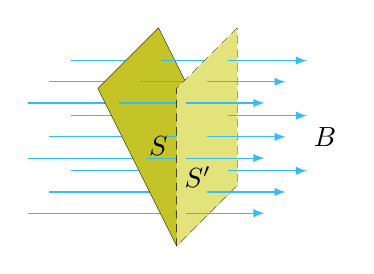
\begin{tikzpicture}[>=latex,scale=1.0]
  % \useasboundingbox(-1,-2)rectangle(8,6);
  \foreach \y in {-0.7,0,0.7}
    \foreach \z in {-0.7,0,0.7}
      { \draw[cyan!80!white] (0,\y,\z)--++(-2,0,0);}
  \fill[yellow8,draw=black,ultra thin](-1,1,-1)--(-1,1,1)--(0,-1,1)--(0,-1,-1)--cycle;
  \foreach \y in {-0.7,0,0.7}
  \foreach \z in {-0.7,0,0.7}
    { \draw[cyan!80!white] (0,\y,\z)--++(-0.5-0.5*\y,0,0);}
  \fill[yellow9,draw=black,ultra thin,densely dashed](0,1,-1)--(0,1,1)--(0,-1,1)--(0,-1,-1)--cycle;
  \foreach \y in {-0.7,0,0.7}
    \foreach \z in {-0.7,0,0.7}
      { \draw[cyan!80!white,->] (0,\y,\z)--++(1,0,0);}
  \node at (1.5,0,0) {$B$};
  \node at (0,-0.4,0.3) {$S'$};
  \node at (-0.5,0,0.3) {$S$};
\end{tikzpicture}
\end{document}